\documentclass[dvipdfmx,uplatex]{beamer}
\usepackage{bxdpx-beamer}

\usefonttheme[onlymath]{serif}
\usepackage{tgheros}
\usepackage[haranoaji]{pxchfon}
\renewcommand{\kanjifamilydefault}{\gtdefault}
\usepackage{jslogo}

\usepackage{pxrubrica}

\usepackage[dvipsnames]{xcolor}
\usepackage{svg}
\usepackage{graphicx}
\usepackage[export]{adjustbox} % Enables the valign option in \includegraphics
\usepackage{amsmath,amssymb}

\usepackage[
  backend=biber,
  style=numeric,
  sorting=none
]{biblatex}

\addbibresource{main.bib}

\makeatletter
\let\mkbibemph=\mkbibitalic
\let\blx@imc@mkbibemph=\blx@imc@mkbibitalic
\makeatother

\setlength{\biblabelsep}{0.5em}

\usetheme{Madrid}

\hfuzz=10pt
\vfuzz=10pt

\title[数学で読み解くピアノの音]{数学で読み解くピアノの音}
\subtitle{周波数解析と平均律・うなりの数学的考察}
\author{楠原 朔}
\date{2 September, 2026 (R8)}

\begin{document}

% タイトル
\begin{frame}
    \maketitle
\end{frame}

% 目次
\begin{frame}{目次}
    \tableofcontents
\end{frame}

\section{研究の目的}

\begin{frame}{研究の目的}
  \begin{block}{研究の概要}
    ピアノが出す音を録音し，波形や周波数スペクトルを用いて音の特徴を分析するとともに，音と数学（平均律・和音・三角関数）の関係について考察する．
  \end{block}

  \begin{itemize}
    \item \textbf{疑問}: なぜ特定の音の組み合わせ（和音）は綺麗に聞こえるのか？
    \item \textbf{課題}: 現代の調律法（平均律）における数学的仕組みと，純正な音程との「誤差」を定量的に評価する．
    \item \textbf{手法}: 録音した音声をWAV形式に変換し，C++とlibsndfileを用いて波形を取得する．
          その後，FFTによって周波数スペクトルを求め，gnuplotで可視化する．
  \end{itemize}
  gnuplotとは，グラフを描画するためのソフトウェアである．
  C++とは，汎用プログラミング言語のひとつである．
  libsndfileとは，音声ファイルを読み書きするためのライブラリである．
  ライブラリとは，プログラムの部品のようなもので，他のプログラムから呼び出して利用することができる．
\end{frame}

\begin{frame}{研究の目的（ことばの補足）}
  \begin{block}{ことばの補足}
    波形とは，音の大きさ（振幅）が時間とともにどう変化するかをグラフにしたものである．

    周波数スペクトルとは，その音にどの高さ（周波数）の音がどれくらいの強さで混ざっているかを表したグラフである．

    三角関数とは，$\sin$や$\cos$のように，音の波のようにくり返す形を表すのに使われる数学の関数である．

    平均律とは，1オクターブを12等分して隣り合う音どうしの高さの差をすべて均等にした，現在のピアノなどで使われる音の決め方である．

    純正律とは，和音が最も美しく響くように，周波数の比を簡単な整数比にして作られた音律のこと．
    純正律比は，音を決めるための具体的な整数比のことを指す．

    平均律が音の間隔を均等にするのに対し，純正律はハーモニーの美しさを重視している．
  \end{block}
\end{frame}

\section{仮説}

\begin{frame}{仮説}

  音を聴いたときの「協和的」「不協和的」という印象には，
  2つの音の周波数の関係が影響していると考えた．

  この場合，「協和的な音」は，複数の音が同時に鳴ったときに互いによく溶け合い，心地よく聞こえる音の組み合わせを指す．
  「不協和的な音」を，同時に鳴らしたときに調和せず，不安定で耳障りな響きを与える音（の組み合わせ）を指す．

  \begin{block}{仮説}

    2つの音の周波数比が，
    $1:2$や$2:3$などの比較的単純な整数比に近いほど，
    協和的に感じられる傾向があるのではないか．

  \end{block}

  また，単純な整数比から離れた組み合わせでは，
  不協和的に感じられる傾向があるのではないかと考えた．

\end{frame}

% 工事しよう, まだ書き途中だ．
% 仮説の次に録音と研究を行う．

\section{前提知識}

\subsection{FFTについて}

\begin{frame}{FFTについて (1/2)}
  「\aruby{高速フーリエ変換}{{Fast}~{Fourier}~{Transform}~=~{FFT}}」とは，
  コンピュータを使って「\aruby{離散フーリエ変換}{{Discrete}~{Fourier}~{Transform}~=~{DFT}}」を非常に速く計算するアルゴリズムである．
  時間や空間の信号を周波数成分に分解する処理の基礎となる．

  \footnotesize
  かんたんに言うと，1つの複雑な音の波を，たくさんの単純な波（純粋な高さの音）の足し算に分解して，
  「どの高さの音がどれくらいの強さで混ざっているか」を調べる計算方法である．
  \normalsize

  \begin{block}{DFTについて}
    \begin{itemize}
      \item 離散フーリエ変換の基本目的: 一定間隔でサンプリングされたデータ（$N$ 個の数値の並び）を，周波数ごとの振幅と位相に変換する．
      \item 特徴: 時間領域と周波数領域の双方が「離散的」かつ「周期的」として扱われる．
      \item 逆変換: 逆離散フーリエ変換（IDFT）により，周波数領域のデータから元の時間領域の波形を完全に復元できる．
    \end{itemize}
  \end{block}
  \footnotesize
  サンプリングとは，一定の時間間隔ごとに音の大きさを数値として記録することである．
  振幅とは音の大きさ，位相とは波の始まりのタイミング（ずれ）を表す．
\end{frame}

\begin{frame}{FFTについて (2/2)}
  \begin{block}{計算量の変化とアルゴリズム}
    \begin{itemize}
      \item 直接計算（DFT）の場合，データ数 $N$ に対して $O(N^2)$ 回の計算が必要になる．\footnote[frame]{$O$（ランダウの記号）: データ数 $N$ が増えたときの計算量の増え方の目安を表す記号．}
      \item 回転因子の周期性や対称性を利用して，計算量を $O(N \log N)$ に劇的に減らすアルゴリズムがFFTである．\footnote[frame]{$\log$（対数）: ここでは底を 2 とする対数（$\log_2 N$）．データを半分に分割していく回数を表す．}
    \end{itemize}
  \end{block}

  \footnotesize
  かんたんに言うと，同じような計算をくり返し使い回すことで，計算のムダを大きく減らす工夫がFFTである．
  たとえば $N$ が10倍になっても，DFTでは計算量がおよそ100倍になるのに対し，FFTでは10倍ちょっとにしかならない．
  \normalsize

  \vspace{0.5em}
  時間や空間の信号処理における計算量を大幅に削減できるため，
  実用的な音声・画像・通信のプログラムでは，ほぼ例外なくこのFFTが使われている．
\end{frame}

\section{録音・分析}

\begin{frame}{録音にあたって}
  自宅には電子オルガンがあるので，録音は電子オルガンを用いて行った．
  録音機器はスマートフォン（iPhone 17e）のマイクを利用し，純正のボイスメモアプリで録音した．

  音声ファイルは，圧縮という処理を行うことで，音質が劣化する場合がある．
  ただ，音質が劣化する代わりに，そのファイルのサイズを小さくすることができる．
  録音する際には，長時間録音するためにファイルサイズを小さくするか，
  音質を重視してファイルサイズを大きくするかの選択が必要である．

  \begin{block}{ボイスメモアプリの設定}
    \begin{itemize}
      \item 録音モード: ステレオ \\
      ステレオを選択することで，左右の音の違いを録音することができる．
      \item オーディオの品質: ロスレス圧縮 \\
      ロスレス圧縮を選択することで，音質を劣化させず容量の圧縮を防げる。
    \end{itemize}
  \end{block}
\end{frame}

\begin{frame}{分析するための確認・変換作業}
  \subsection{録音したファイルの確認}
  \small
  録音したファイルを，PCに取り込み，ffmpegというソフトウェアを用いて変換することにする．
  ffmpegとは，マルチメディアファイルを処理するためのオープンソースのツールである．
  GUIというウィンドウで操作せず，各OSのコマンドラインで操作するソフトウェアである．
  Windowsにおいて，Powershellやコマンドプロンプトがプリインストールされている．
  ただ，今回は学校のPCで作業するため，
  ソフトウェアのインストールに関する規制を回避するため，
  Windows上でLinuxのような開発環境などを使えるようにする，
  msys2というソフトウェアツール群を用いることにする．
  msys2では，pacmanというパッケージ管理・追加システムを用いて多くのパッケージをインストールすることができる．

  \footnotesize
  オープンソースとは，プログラムの中身（設計図にあたるもの）が誰でも見られるように公開されていることをいう．
  コマンドラインとは，ボタンをクリックする代わりに，文字で命令を入力してコンピュータを操作する方法である．
  \normalsize
  \begin{figure}[htbp]
    \centering
    % \includegraphics[scale=0.24, valign=t]{pictures/mingw64.png}
    % msys2 mingw64のロゴは著作権などの関係上、問題の可否が不明なため削除します。
    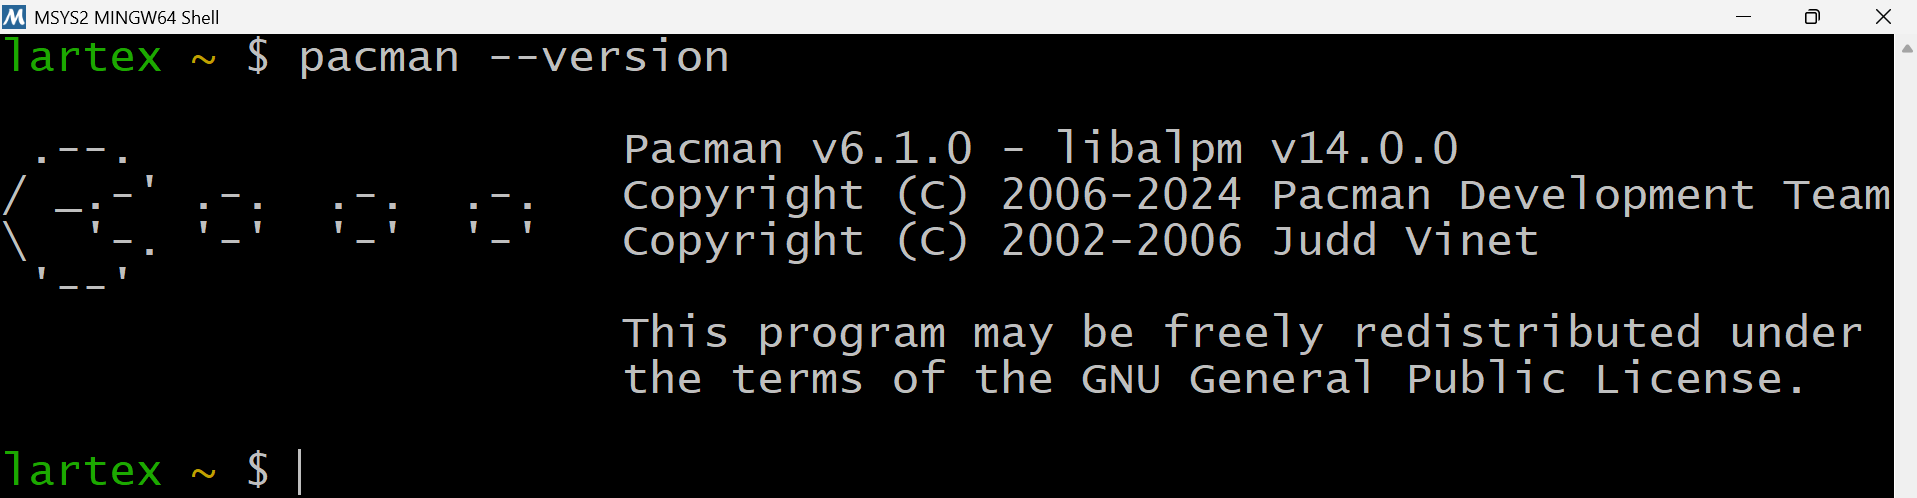
\includegraphics[scale=0.15, valign=t]{pictures/pacman.png}
  \end{figure}
\end{frame}

\begin{frame}
    \begin{block}{拡張子について}
    拡張子とは，ファイル名の末尾に付けられる文字列で，ファイルの種類を示すものである．
    音声ファイルの拡張子には，wav，mp3，flacなどがある．
    \begin{itemize}
      \item mp3は，音声データを圧縮するための形式であり，圧縮率が高く，ファイルサイズが小さいために，劣化してしまう．
      \item wavは，音声データを非圧縮で保存する形式であり，音質は劣化しないが，ファイルサイズが大きい．
      \item m4aは，Apple社が開発した音声ファイル専用の記録形式で，一般的にMP3よりも高音質かつファイルサイズが小さく抑えられる特徴がある．
    \end{itemize}
    今回はそのffmpegで，m4a形式のファイルをwav形式に変換することにする．
  \end{block}
\end{frame}

\begin{frame}{FFT/DFTと今回行う分析を絡める}
  FFT/DFTを行う前の音声ファイル，今回で言う変換したwav形式のファイルは，
  「時刻 t のとき，マイクの振幅はいくつだったか」を表すデータである．
  そのwav形式の音声ファイルをFFT/DFTにかけることで，
  「\aruby{周波数 f}{{frequency}} の振動が，どのくらい含まれているか」を表すデータに変換することができる．

  ただ，FFT/DFTを実行させるためのプログラムを作らなければならず，
  そのためにはプログラミング言語を学習し，用いる必要性がある．
  なお，最近は生成AIの発展により，プログラミング言語を学習せずとも，
  生成AIにプログラムを作成してもらうことが可能になった．
  今回は，生成AIにプログラムを作成してもらい，FFT/DFTを行うプログラムを作成した．
  生成AI: Anthropic Claude Sonnet 5
\end{frame}

\section{結果を見るための前提知識}

\begin{frame}{音名について}
  \small

  今回扱うのは，電子オルガンの音であり，ピアノの音と同じ音名を持つ．
  音名は，アルファベットの大文字と数字の組み合わせで表されることが多い．

  \begin{minipage}{0.48\textwidth}
    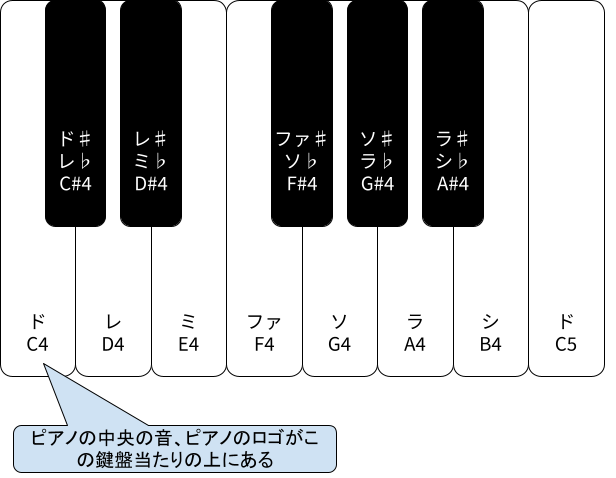
\includegraphics[width=0.85\textwidth]{pictures/piano.png}
    \footnotesize{十二平均律として用いられるピアノの鍵盤と音}
  \end{minipage}
  \hfil
  \begin{minipage}{0.47\textwidth}
   \begin{itemize}
      \item C, D, E, F, G, A, B：音名
      \item 数字：オクターブを表す
      \item $\sharp$：その音を半音高くする記号
   \end{itemize}

  \begin{block}{今回の研究で単音として扱う音}
    単音とは，1つの音名で表される音のこと．
    C4, D4, E4, F4, G4, A4, B4, C5
  \end{block}
  \end{minipage}

  例えば，C4の次に高い白鍵はD4であり，
  C4からC5までにはC4, D4, E4, F4, G4, A4, B4, C5の8音がある．

  1オクターブとは，C4からC5までの8音のことを指し，周波数はちょうど2倍になる関係のことである．

  \footnotesize
  半音とは，鍵盤の隣どうしの音の高さの差のことである．
\end{frame}

\begin{frame}{用語集}
  \small

  \begin{block}{理論周波数}
    平均律の式から計算される，その音の周波数．
  \end{block}

  \begin{block}{実測周波数}
    録音した音声をDFTで周波数解析し，
    対象となる音の理論周波数付近で観測されたピークの周波数．
  \end{block}

  今回は，録音した音声そのものを測定するため，
  理論値と実測値が完全に一致するとは限らない．

  \begin{block}{cent（セント）}
    音程の差を細かく表すための単位．
    1オクターブを1200 centとして，
    半音(1つの鍵盤間)は100 centに相当する．
  \end{block}

  \footnotesize
  セントとは，音の高さのわずかなズレを細かく測るための「ものさし」のような単位である．
  \normalsize

  したがって，理論値と実測値の差を
  Hzだけでなくcentでも比較する．

\end{frame}

\section{結果}

\begin{frame}{録音した単音の音声}
  \begin{itemize}
    \item 理論周波数: 従来の周波数
    \item 実測周波数: 録音した音声をDFTで解析した結果の周波数
    \item Hz誤差: 理論周波数$-$実測周波数
    \item cent誤差: 理論周波数と実測周波数の差をcentで表したもの
  \end{itemize}
\begin{table}[!ht]
    \centering
    \begin{tabular}{|l|l|l|l|l|}
    \hline
        音名 & 理論周波数 & 実測周波数 & Hz誤差 & cent誤差 \\ \hline
        %L13 & L13 & L58 & L59 & L61 \\ \hline
        %note & theoretical\_frequency\_hz & measured\_frequency\_hz & error\_hz & cent\_error \\ \hline
        C4 & 261.625565 & 260.742188 & -0.883377 & -5.855397 \\ \hline
        D4 & 293.664768 & 292.968750 & -0.696018 & -4.108086 \\ \hline
        E4 & 329.627557 & 328.125000 & -1.502557 & -7.909607 \\ \hline
        F4 & 349.228231 & 348.632812 & -0.595419 & -2.954198 \\ \hline
        G4 & 391.995436 & 392.578125 & 0.582689 & 2.571515 \\ \hline
        A4 & 440.000000 & 439.453125 & -0.546875 & -2.153085 \\ \hline
        B4 & 493.883301 & 495.117188 & 1.233887 & 4.319810 \\ \hline
        C5 & 523.251131 & 524.414062 & 1.162931 & 3.843419 \\ \hline
    \end{tabular}
\end{table}
\end{frame}

\begin{frame}{周波数解析の結果}
  C4の録音音声をDFTで解析したところ，N=4096では$257.8125$ Hzに最大ピークが現れた．N=16384では周波数分解能が向上し，$260.742188$ Hzに最大ピークが現れた．C4の理論値$261.625565$ Hzとの差は，N=4096では$-3.813$ Hzであったのに対し，N=16384では$-0.883$ Hzまで小さくなった．

  \footnotesize
  周波数分解能とは，どれだけ細かく周波数を区別できるかを表す指標である．
  DFTに使うデータの数（サンプル数）$N$を増やすほど，1つ1つの目盛りが細かくなり，より正確に音の高さを求めることができる．
\end{frame}

\begin{frame}{3和音の周波数解析}

  C4--E4--G4の和音を録音し，DFTで周波数解析を行った．

  \begin{table}[!ht]
    \centering
    \begin{tabular}{|c|r|r|r|}
      \hline
      音名 & 理論周波数(Hz) & 実測周波数(Hz) & cent誤差 \\ \hline
      C4 & 261.625565 & 260.742188 & -5.855397 \\ \hline
      E4 & 329.627557 & 328.125000 & -7.909607 \\ \hline
      G4 & 391.995436 & 392.578125 & 2.571515 \\ \hline
    \end{tabular}
  \end{table}

  \begin{itemize}
    \item C4，E4，G4それぞれの理論周波数付近にピークが観測された．
    \item 単音の場合とは異なり，1つの録音から複数の周波数成分を確認できた．
    \item したがって，和音は周波数スペクトル上でも複数の音の成分として観測できる．
  \end{itemize}

\end{frame}

\begin{frame}{和音について}

  今回は，2つの異なる音を同時に鳴らして録音した．

  \begin{block}{和音}
    複数の異なる高さの音を同時に鳴らしたものを和音という．
  \end{block}

  実際に音を聴き比べると，
  音の組み合わせによって「よく響く音」と
  「濁って聞こえる音」があるように感じられる．

  \begin{itemize}

    \item よく響いて聞こえる組み合わせ；音同士がよく調和し，安定して聴こえる響き

    $\rightarrow$ 協和的な響き，協和音，協和音程

    \item 濁って聞こえる組み合わせ；音同士がぶつかり合うように感じられ，緊張感や濁り，不安定さを感じる響き

    $\rightarrow$ 不協和的な響き，不協和音，不協和音程

  \end{itemize}

  ただし，協和・不協和を明確な境界によって完全に二分できるとは限らない．
  そこで，本研究では特定の組み合わせを「協和音」「不協和音」と断定せず，
  音を聴いた際の響き方が完全に「協和音」であると言い切れない場合に，\textbf{傾向}として扱うことにする．

\end{frame}

\begin{frame}{今回録音した2音の組み合わせ}

  C4を基準として，次の音との組み合わせを録音した．

  \begin{table}[!ht]
    \centering
    \begin{tabular}{c|c}
      \hline
      番号 & 組み合わせ \\ \hline
      18 & C4--C$\sharp$4 \\
      19 & C4--D4 \\
      20 & C4--D$\sharp$4 \\
      21 & C4--E4 \\
      22 & C4--F4 \\
      23 & C4--F$\sharp$4 \\
      24 & C4--G4 \\
      25 & C4--G$\sharp$4 \\
      26 & C4--A4 \\
      27 & C4--A$\sharp$4 \\
      28 & C4--B4 \\
      29 & C4--C5 \\
      \hline
    \end{tabular}
  \end{table}

  要するに，真ん中のドから，一オクターブ上の音までを，半音ずつ順番に組み合わせて録音したということ．

\end{frame}

\begin{frame}{2音の周波数解析結果}

\begin{table}[!ht]
    \centering
    \begin{tabular}{|l|l|l|l|l|}
    \hline
        音名 & 2音目理論値 & 2音目実測値 & 2音目cent誤差 & 聴き心地 \\ \hline
        C4-C$\sharp$4 & 277.182631 & 275.390625 & -11.23 & 良くない \\ \hline
        C4-D4 & 293.664768 & 292.96875 & -4.11 & 独特な \\ \hline
        C4-D$\sharp$4 & 311.126984 & 310.546875 & -3.23 & 若干協和的 \\ \hline
        C4-E4 & 329.627557 & 328.125 & -7.91 & 若干協和的 \\ \hline
        C4-F4 & 349.228231 & 348.632812 & -2.95 & 協和的 \\ \hline
        C4-F$\sharp$4 & 369.994423 & 369.140625 & -4 & 不気味な \\ \hline
        C4-G4 & 391.995436 & 392.578125 & +2.57 & 協和的 \\ \hline
        C4-G$\sharp$4 & 415.304698 & 416.015625 & +2.96 & 若干協和的 \\ \hline
        C4-A4 & 440 & 439.453125 & -2.15 & 若干協和的 \\ \hline
        C4-A$\sharp$4 & 466.163762 & 465.820312 & -1.28 & 緊張感 \\ \hline
        C4-B4 & 493.883301 & 495.117188 & +4.32 & 良くない \\ \hline
        C4-C5 & 523.251131 & 524.414062 & +3.84 & 協和的 \\ \hline
    \end{tabular}
\end{table}

全て2音目の結果である．1音目であるC4の理論値は261.625565，実測値は260.742188である．cent誤差は-5.855397である．

\end{frame}

\begin{frame}
  ここで，録音した2音による和音について，
  1つ目の単音と2つ目の単音の周波数比を算出する．
  実測した周波数比を，近い単純な整数比で近似する．
  なお，録音時の測定誤差を考慮し，
  一定の許容範囲内で最も簡潔な整数比に近似する処理を行った．

  \begin{table}[!ht]
    \centering
    \begin{minipage}{0.6\textwidth}
      \centering
      \scalebox{1}{
        \begin{tabular}{|l|l|l|}
        \hline
            音名 & 純正律比 & うなり周波数 \\ \hline
            C4-C$\sharp$4 & 15:16 & 41.016 \\ \hline
            C4-D4 & 8:9 & 2.93 \\ \hline
            C4-D$\sharp$4 & 5:6 & 11.719 \\ \hline
            C4-E4 & 4:5 & 8.789 \\ \hline
            C4-F4 & 3:4 & 2.93 \\ \hline
            C4-F$\sharp$4 & 32:45 & 79.102 \\ \hline
            C4-G4 & 2:3 & 2.93 \\ \hline
            C4-G$\sharp$4 & 5:8 & 5.859 \\ \hline
            C4-A4 & 3:5 & 14.648 \\ \hline
            C4-A$\sharp$4 & 9:16 & 20.508 \\ \hline
            C4-B4 & 8:15 & 49.805 \\ \hline
            C4-C5 & 1:2 & 2.93 \\ \hline
        \end{tabular}
      }
    \end{minipage}%
    \hfill
    \begin{minipage}{0.35\textwidth}
      
      うなり周波数（あるいは，うなりの振動数）とは，
      わずかに異なる周波数の2つの波が重なり合うとき，
      音量の上下する変化の速さのこと．

      一般的な定義では\\
      $ f = |f_1 - f_2| $
      である．今回は，
      2つの音($f_1, f_2$)が理論上の単純な整数比$p:q$($\frac{f_2}{f_1} \approx \frac{p}{q}$)に近いとき，
      \[ \text{beat\_hz} = |q \cdot f_2 - p \cdot f_1| \]
      として算出する．

    \end{minipage}
  \end{table}
\end{frame}

\begin{frame}{純正律比との比較}

  今回録音した2音の組み合わせについて，
  今回算出した周波数比と，
  純正律で用いられる周波数比を比較した．

  そして，東芝吹奏楽団による
  「純正律の具体的な利用法について」\cite{junseiritu}を参照し，
  今回算出した周波数比と比較した．

  \begin{itemize}

    \item C4--F4：3:4，周波数が$\frac{4}{3}$倍，完全四度

    \item C4--G4：2:3，周波数が$\frac{3}{2}$倍，完全五度

    \item C4--C5：1:2，周波数が$2$倍，完全八度（一オクターブ）

  \end{itemize}

  今回の解析結果では，これらの比較的単純な整数比を持つ
  組み合わせは，実際に聴いた際にも協和的に感じられた．

\end{frame}

\section{考察}

\begin{frame}{考察}

  今回，電子オルガンの音を録音し，
  DFTによる周波数解析を行った結果，
  理論周波数に近い周波数ピークを確認することができた．

  また，2音を同時に鳴らした場合について，
  実際に聴いた際の印象と周波数比を比較した．

  その結果，

  \begin{itemize}

    \item C4--F4：$3:4$

    \item C4--G4：$2:3$

    \item C4--C5：$1:2$

  \end{itemize}

  のように，比較的単純な整数比を持つ組み合わせは，
  今回の実験では協和的に感じられる傾向が見られた．

  一方で，協和・不協和の感じ方には個人差や演奏方法，
  楽器の音色なども影響すると考えられるため，
  周波数比だけによって完全に決定されるとは限らない．

\end{frame}

\section{まとめ}

\begin{frame}{まとめ}

  \begin{itemize}

    \item 録音した電子オルガンの音をWAV形式に変換し，
    DFTによる周波数解析を行った．

    \item 単音および複数の音を同時に鳴らした録音から，
    それぞれの音に対応する周波数成分を確認できた．

    \item DFTのサンプル数を増やすことで，
    周波数分解能が向上することを確認した．

    \item 2音の組み合わせを比較した結果，
    $3:4$，$2:3$，$1:2$などの比較的単純な整数比を持つ
    組み合わせでは，協和的に感じられる傾向が見られた．

  \end{itemize}

  今回の研究を通して，普段何気なく聴いているピアノの音にも，
  周波数や数学的な規則性が関係していることを確認できた．

\end{frame}

\section{感想}

\begin{frame}{感想}

  今回の研究では，私（たち）が普段何気なく聴いている音を，
  周波数という目に見える数値とグラフに変換して，分析することができた．

  特に，実際には同じように聞こえていた音でも，
  DFTによって周波数を調べることで，
  理論値との違いや音同士の周波数比を
  具体的な数値として確認できたことが印象に残った．

  また，協和的・不協和的に感じる音の組み合わせについても，
  単純な「良い音・悪い音」というだけではなく，
  周波数比やうなりなどの数学的な要素から
  考えることができた．

  音楽と数学は別々のものだと思っていたが，
  実際に音を解析してみることで，
  数学が音楽の中にも関係していることを実感した．

  また，不協和音というもの自体は，悪いものではなく，緊張感を生み出したり，
  うまい感じに不協和音をひたすらに並べた曲もあることから，音楽の奥深さを感じた．

\end{frame}

\section{参考文献}

\begin{frame}{参考文献}
    \printbibliography[heading=none]
    \nocite{wasei}
    \nocite{chart}
\end{frame}

\makeatletter
\def\eupTeX{
  $\m@th\varepsilon$-\upTeX
}

\makeatother

\section{謝辞}

\begin{frame}{謝辞}

  本研究では，音声解析や資料作成にあたり，多くのソフトウェアや開発環境を利用しました．
  これらのソフトウェア，フォントおよび関連する開発者・関係者の皆様に感謝いたします．
  
  原稿製作にあたって
  \begin{itemize}
    \item \TeX Live 2025, up\LaTeX (at \eupTeX ), synctex, dvipdfmx
    \item \LaTeX\ with Beamer class
    \item Hyperref, \textsc{bib\LaTeX}, Biber
  \end{itemize}

  解析ウェアを製作するにあたって
  \begin{itemize}
    \item msys2 ucrt64
    \item toolchain (C++), libsndfile, ffmpeg
    \item GitHub Copilot
  \end{itemize}

  本原稿の内部で使用したフォント類
  \begin{itemize}
    \item 原ノ味ゴシック
    \item TeX Gyre Heros (及び原本となったAdobe35書体中のHelvetica)
    \item Computer Modern Family (Roman, Math Italic, Typewriter, Symbol)
    \item Latin Modern Family (Roman)
  \end{itemize}

  ありがとうございました

\end{frame}

\section{終わりに}

\begin{frame}{終わりに}
  \centering
  \Huge{ご清聴ありがとうございました}
\end{frame}

\end{document}